\documentclass[10pt, a4paper, italian]{article}
\usepackage[T1]{fontenc}
\usepackage[utf8]{inputenc}
\usepackage{amsmath, amssymb, amsthm, thmtools, amsfonts, mathtools}
\usepackage{nicefrac}
\usepackage{calc}
\usepackage[pdftex, hyperindex, plainpages=false]{hyperref}
\usepackage[nameinlink]{cleveref} %load before classicthesis (clash)
%\usepackage[nochapters,pdfspacing]{classicthesis}
\usepackage{siunitx}
\usepackage[siunitx]{circuitikz}

\usepackage[a4paper]{geometry}
\usepackage{float}
\usepackage{mdframed}
\usepackage{titling}
\usepackage{booktabs}
\usepackage{graphicx}
\usepackage{caption, subcaption}
\usepackage{xcolor}
\usepackage[italian]{babel}
\usepackage{pgfplots}
\usepackage{listings}
%\usepackage{lmodern}
\usepackage{url}
\usepackage{enumitem}
\usepackage{tikz} %loads after classicthesis (xcolor incompat)

% lets graphicx know path where figures to be included are found
\graphicspath{{../figs/}}
\makeatletter
\def\input@path{{../figs/}}
%or: \def\input@path{{/path/to/folder/}{/path/to/other/folder/}}
\makeatother

% tikz pgf plots setup
\usepgfplotslibrary{external}
\pgfplotsset{compat=1.15}
%\tikzexternalize

% spaces and significant digits/figures for measurements
\sisetup{free-standing-units, space-before-unit, number-unit-product = \;,
scientific-notation = false, round-mode = figures, round-precision = 1,}

% turns all (hyperlinked) references black [default is blue]
\hypersetup{
	linktoc=all,
	colorlinks=true,
	linkcolor=black
}

% code listings config
%\lstset{
%language=Python,
%basicstyle=\ttfamily,
%columns=fullflexible,
%keepspaces=true,
%}

% mdframed (for boxed text) configuration
\mdfsetup{linewidth=0.6pt}

% Default fixed font does not support bold face
\DeclareFixedFont{\ttb}{T1}{txtt}{bx}{n}{12} % for bold
\DeclareFixedFont{\ttm}{T1}{txtt}{m}{n}{12}  % for normal

% Custom colors
\usepackage{color}
\definecolor{deepblue}{rgb}{0,0,0.5}
\definecolor{deepred}{rgb}{0.6,0,0}
\definecolor{deepgreen}{rgb}{0,0.5,0}

% Commands 
\newcommand{\executeiffilenewer}[3]{%
	\ifnum\pdfstrcmp{\pdffilemoddate{#1}}%
		{\pdffilemoddate{#2}}>0%
	{\immediate\write18{#3}}\fi%
}
% input .svg --> .pdf_tex graphs
%\newcommand{\includesvg}[1]{%
%	\executeiffilenewer{#1.svg}{#1.pdf}%
%	{inkscape -z -D --file=#1.svg %
%	--export-pdf=#1.pdf --export-latex}%
%	\input{#1.pdf_tex}%
%}
% Thanks UniPi's Department of Physics E. Fermi
\newcommand{\thanksdf}{(\thanks{Dipartimento di Fisica E.~Fermi,%
Universit\`a di Pisa - Pisa, Italy.}\;)}

% hyperlink to email address
\newcommand{\mail}[1]{\href{mailto:#1}{\textsf{#1}}}

% \vec for bold vectors, instead of overarrows (now "\arrvec")
\let\arrvec=\vec
\renewcommand{\vec}[1]{\boldsymbol #1}
% replaces straight phi with slanted phi
\renewcommand{\phi}{\varphi}
% replaces straight eps with curved epsilon
\newcommand{\eps}{\varepsilon}
% abbreviation for (sub_/super^)scripts of \lim, \sum,... in inline math
\newcommand{\ds}{\displaystyle}

% blackboard/number set letters
\newcommand{\CC}{\mathbb C}
\newcommand{\HH}{\mathbb H}
\newcommand{\KK}{\mathbb K}
\newcommand{\NN}{\mathbb N}
\newcommand{\PP}{\mathbb P}
\newcommand{\QQ}{\mathbb Q}
\newcommand{\RR}{\mathbb R}
\newcommand{\ZZ}{\mathbb Z}

\newcommand{\Abs}[1]{{\left\Vert #1\right\Vert}}
\newcommand{\enclose}[1]{{\left( #1 \right)}}
\newcommand{\Enclose}[1]{{\left[ #1 \right]}}
\newcommand{\floor}[1]{\left\lfloor #1 \right\rfloor}
\newcommand{\ceil}[1]{\left\lceil #1 \right\rceil}
\newcommand{\To}{\rightrightarrows}

% Math operators
\DeclareMathOperator{\divergence}{div}
\renewcommand{\div}{\divergence}
\DeclareMathOperator{\Imaginarypart}{Im}
\renewcommand{\Im}{\Imaginarypart}
\DeclareMathOperator{\Realpart}{Re}
\renewcommand{\Re}{\Realpart}
%\DeclareMathOperator{\arg}{arg}
\DeclareMathOperator{\tg}{tg}
\DeclareMathOperator{\arctg}{arctg}
\DeclareMathOperator{\settsinh}{settsinh}
\DeclareMathOperator{\settcosh}{settcosh}
\DeclareMathOperator{\tr}{tr}
\DeclareMathOperator{\im}{im}
\DeclareMathOperator{\sgn}{sgn}
\DeclareMathOperator{\diag}{diag}

\DeclarePairedDelimiter{\norm}{\lVert}{\rVert}
\DeclarePairedDelimiter{\scalar}{\langle}{\rangle}

% Logarithm with arbitrary base.
% -> log_10
\newcommand{\llog}[1][10]{\log_{#1}}

% Absolute value.
% -> |x|
\newcommand{\abs}[1]{\left| #1 \right|}

% Powers.
% -> x^a
\newcommand{\power}[2][2]{\left( #2 \right)^{#1}}

% Square.
% -> x^2
\newcommand{\sq}[1]{\power[2]{#1}}

% Expansion of the binomial coefficient.
% -> n1!/(n2!(n1 - n2)!)
\newcommand{\binomexpr}[2]{\frac{#1!}{#2!(#1 - #2)!}}

% Expression evaluation at a given point with square brackets.
% -> [x]_{a}
\newcommand{\at}[2]{\left[ #1\right]_{\makebox[-1pt][l]{${\scriptstyle#2}$}}}

% Expression evaluation in an interval.
% -> [x] _{a}^{b}
\newcommand{\eval}[3]{\left.#1%
  \right|_{\makebox[-1pt][l]{${\scriptstyle#2}$}}^{\makebox[-1pt][l]{${\scriptstyle#3}$}}}

% Upright d in math mode (for differentials).
% -> d
\newcommand{\ud}{\mathrm{d}}

% Differential.
% -> dx
\newcommand{\diff}[1][x]{\,\ud{#1}}

% Base command for defining derivatives.
% -> df/dx or d^kf/dx^k
\newcommand{\basederivative}[4][]{%
  \displaystyle%
  \ifx\\#1\\\frac{#4#2}{#4#3}%
  \else%
  \frac{#4^#1#2}{#4#3^#1}%
  \fi%
}

% Total derivative.
% -> df/dx(x) or d^kf/dx^k(x)
\newcommand{\td}[4][]{%
  \basederivative[#1]{#2}{#3}{\ud}%
  \ifx\\#4\\%
  \else%
  \mkern-4mu\left(#4\right)%
  \fi%
}

% Partial derivative.
% -> df/dx(x) or d^kf/dx^k(x)
\newcommand{\pd}[4][]{%
  \basederivative[#1]{#2}{#3}{\partial}%
  \ifx\\#4\\%
  \else%
  \mkern-4mu\left(#4\right)%
  \fi%
}

\newcommand{\intinf}{\int_{-\infty}^{\infty}\!\!\!}

\newcommand{\cinterval}[2]{\left[\, #1,~#2 \,\right]}

\newcommand{\linterval}[2]{\left[\, #1,~#2 \,\right)}

\newcommand{\rinterval}[2]{\left(\, #1,~#2 \,\right]}

\newcommand{\ointerval}[2]{\left(\, #1,~#2 \,\right)}

\newcommand{\prob}[1]{\displaystyle P\left(#1\right)}

\newcommand{\pvalue}{\emph{$p$-value}}

\newcommand{\cond}{\,|\,}

\newcommand{\expect}[1]{\displaystyle E\left[#1\right]}

\newcommand{\mom}[2][]{\displaystyle {\cal M}_{#2}\ifx\\#1\\\else(#1)\fi}

\newcommand{\momalg}[1]{\displaystyle \lambda_{#1}}

\newcommand{\momcen}[1]{\displaystyle \mu_{#1}}

\newcommand{\skewness}{\displaystyle \gamma_1}

\newcommand{\kurtosis}{\displaystyle \gamma_2}

\newcommand{\charf}[1][x]{\phi_{#1}}

\newcommand{\momgenf}[1][x]{M_{#1}}

\newcommand{\fwhm}{{\scriptstyle \textsc{FWHM}}}

\newcommand{\hwhm}{{\scriptstyle \textsc{HWHM}}}

\newcommand{\median}{\mu_{\nicefrac{1}{2}}}

\newcommand{\var}[1]{\ensuremath{\text{Var}\left(#1\right)}}

\newcommand{\cov}[2]{\ensuremath{\text{Cov}\left(#1, #2\right)}}

\newcommand{\corr}[2]{\ensuremath{\text{Corr}\left(#1, #2\right)}}

\newcommand{\like}{\mathcal L}

\newcommand{\likelihood}[2][]{\like\ifx\\#2\\\else(#2\ifx\\#1\\\else;#1\fi)\fi}

\newcommand{\chisq}{\ensuremath{\chi^2}}

\newcommand{\chisquare}[2][]{\chisq\ifx\\#2\\\else(#2\ifx\\#1\\\else;#1\fi)\fi}

\newcommand{\loglikelihood}[2][]{\log\likelihood[#1]{#2}}

\newcommand{\pdf}[3][]{#2(#3\ifx\\#1\\\else;#1\fi)}

\newcommand{\binomialpdf}[2][]{\pdf[#1]{\mathcal B}{#2}}

\newcommand{\multinomialpdf}[2][]{\pdf[#1]{\mathcal M}{#2}}

\newcommand{\poissonpdf}[2][]{\pdf[#1]{\mathcal P}{#2}}

\newcommand{\uniformpdf}[2][]{\pdf[#1]{u}{#2}}

\newcommand{\exponentialpdf}[2][]{\pdf[#1]{\varepsilon}{#2}}

\newcommand{\gausspdf}[2][]{\pdf[#1]{N}{#2}}

\newcommand{\chisquarepdf}[2][]{\pdf[#1]{\wp}{#2}}

\newcommand{\cauchypdf}[2][]{\pdf[#1]{c}{#2}}

\newcommand{\erf}[1]{\ensuremath{\text{erf}\left(#1\right)}}

\newcommand{\dccases}[4][]{#2 \ifx\\#2\\\else=\fi %
  \begin{cases}
    \displaystyle #3 & \text{per variabili discrete}\\
    \displaystyle #4 & \text{per variabili continue}#1
  \end{cases}
}
% sub/super-scriptable for all symbol as math operator 
\newcommand\Scaleforall[1]{\vcenter{\hbox{\scalefont{#1}$\forall$}}}

\DeclareMathOperator*\forevery{%
  \vphantom\sum
  \mathchoice{\Scaleforall{2}}{\Scaleforall{1.4}}{\Scaleforall{1}}{\Scaleforall{0.75}}}
\usepackage{multicol}
\geometry{left=2cm, right=2cm, top=2cm, bottom=2cm}
\usepackage{colortbl}
\usepackage{diagbox}
\usepackage[T1]{fontenc}
\usepackage[utf8]{inputenc}
\usepackage{graphicx}
\usepackage{xcolor}
\usepackage{listings}

\lstset{%
  language = Octave,
  backgroundcolor=\color{white},   
  basicstyle=\footnotesize\ttfamily,       
  breakatwhitespace=false,         
  breaklines=true,                 
  captionpos=b,                   
  commentstyle=\color{gray},    
  deletekeywords={...},           
  escapeinside={\%*}{*)},          
  extendedchars=true,              
  frame=single,                    
  keepspaces=true,                 
  keywordstyle=\color{orange},       
  morekeywords={*,...},            
  numbers=left,                    
  numbersep=5pt,                   
  numberstyle=\footnotesize\color{gray}, 
  rulecolor=\color{black},         
  rulesepcolor=\color{blue},
  showspaces=false,                
  showstringspaces=false,          
  showtabs=false,                  
  stepnumber=2,                    
  stringstyle=\color{orange},    
  tabsize=2,                       
  title=\lstname,
  emphstyle=\bfseries\color{blue}%  style for emph={} 
} 

%% language specific settings:
\lstdefinestyle{Arduino}{%
    language = Octave,
    keywords={void, int boolean},%                 define keywords
    morecomment=[l]{//},%             treat // as comments
    morecomment=[s]{/*}{*/},%         define /* ... */ comments
    emph={HIGH, OUTPUT, LOW}%        keywords to emphasize
}
\usepackage{tkz-graph}
\usepackage{arydshln}
\usetikzlibrary{automata, positioning, arrows}
\newenvironment{FSM}{
\begin{tikzpicture}
\tikzset{
->, % makes the edges directed
>=stealth', % makes the arrow heads bold
node distance=2cm, % specifies the minimum distance between two nodes. Change if necessary.
every state/.style={minimum size = 1cm, thick, fill=gray!10}, % sets the properties for each 'state' node
}
}{
\end{tikzpicture}
}

% indexes subsections with letters, sections with numbers (1.a, 1.b, ...)
\renewcommand{\thesubsection}{\thesection.\alph{subsection}}

% lets graphicx know path where figures to be included are found
\graphicspath{{../figs/}}

\newcommand{\dontcare}{X}
\author{Gruppo 1.AC \\ Matteo Rossi, Bernardo Tomelleri}
\title{EsD3: Macchine a stati finiti: semafori e riconoscitore di fronti}
\begin{document}
\date{\today}
\maketitle

\section{Misura componenti dei circuiti}
Riportiamo per completezza il valore della tensione continua di
alimentazione per i circuiti integrati misurata con il multimetro
\[
V_{CC} = 4.99 \pm 0.03 \; \si{\V}
\]

e il valore di capacità del condensatore di disaccoppiamento che collega le
linee di alimentazione a massa (sempre misurato con il multimetro)
\[
C_d = 97 \pm 4 \; \si{n\F}
\]

%=======================
\section{Implementazione di un semaforo con circuiti integrati}\label{sec: IC}
Si vuole costruire una macchina a stati finiti in grado di emulare il
funzionamento delle luci di un semaforo stradale, nelle modalità
\begin{description}
\item[ABILITATO] si ripetono ciclicamente gli stati: LED verde acceso $\to$
LED giallo e verde accesi $\to$ LED rosso acceso.
\item[DISABILITATO] si alternano gli stati LED giallo acceso e spento
(giallo lampeggiante).
\end{description}
in cui tutti gli stati hanno durata pari ad un impulso del clock inviato
all'ingresso dei circuiti integrati a disposizione.

\subsection{Diagramma a stati del semaforo}
Quando il semaforo è in modalità ``abilitato'' ($E=1$) si susseguono
ciclicamente 3 possibili output, per cui sono stati implementarli con $3$ stati
interni della macchina. Mentre nel caso di semaforo ``disabilitato'' ($E=1$) i
possibili output si riducono a $2$, e si possono esprimere utilizzando due
degli stati precedentemente codificati a seconda del valore logico dell'input
ENABLE tramite un circuito FSM di Mealy.

Scegliamo di codificare con due bit di memoria $(Q_{1} Q_{0})$ i tre stati:
$00$, $01$ e $10$ che corrispondono, quando $E=1$, ai tre output ``verde''
$(V)$, ``verde-giallo'' $(VG)$, ``rosso'' $(R)$. Quando invece $E=0$ vengono
usati solamente i primi due $00$ e $01$, che corrispondono agli output del
semaforo ``spento'' $(Y^0)$ e ``giallo'' $(Y^1)$ come si può vedere già nel
diagramma a stati riportato in \cref{diag: semf}.
\begin{figure}[htbp]
\centering
\begin{FSM}
\tikzset{
    LabelStyle/.style = {
        rectangle, rounded corners, draw,
        minimum width = 1em,
    },
    EdgeStyle/.append style = {-stealth}
}

   \node[state with output] (V) {$V/Y^0$ \nodepart{lower} $00$};
   \node[state with output, right of=V, xshift=2cm] (VG)
   {$VG/Y^1$ \nodepart{lower} $01$};
   \node[state with output, right of=VG, xshift=2cm] (R)
   {$R$ \nodepart{lower} $10$};
   
   \Edge[label = E](V)(VG)
   \Edge[label = E](VG)(R)

\tikzset{EdgeStyle/.append style = {-stealth, bend right = 30}}
   \Edge[label = D](VG)(V)
   \Edge[label = D](V)(VG)

\tikzset{EdgeStyle/.append style = {bend right = 50}}
   \Edge[label = E](R)(V)

\tikzset{EdgeStyle/.append style = {bend left = 50}}
   \Edge[label = D](R)(V)
\end{FSM}
\caption{Diagramma degli stati del semaforo FSM di Mealy con Enable
\label{diag: semf}}
\end{figure}

\subsection{Codifica degli stati della macchina}
La codifica in termini di bit degli stati della macchina è riassunta nella
\cref{tab: bit}, dove $Q_0$ e $Q_1$ corrispondono rispettivamente
al valore logico delle uscite del primo e del secondo flip-flop, mentre $S_E$
e $S_D$ rappresentano lo stato associato al semaforo a seconda che questo sia
ENABLED o DISABLED.
\begin{table}[htbp]
	\centering
	\begin{tabular}{cc|cc}
	\toprule
	$S_D$ &	$S_E$ & $Q_1$ &	$Q_0$ \\
	\midrule
	\midrule
	$Y^0$ & $V$  & $0$	&	$0$	\\
	$Y^1$ & $VG$ & $0$	&	$1$	\\
	 	  & $R$  & $1$	&	$0$	\\
	\bottomrule
	\end{tabular}
	\caption{Codifica binaria scelta per gli stati del semaforo.
	\label{tab: bit}}
\end{table}

\subsection{Tabelle di verità}
Come visto nel diagramma degli stati il segnale di input ENABLE modifica
l'uscita del circuito in maniera asincrona, mentre dalla tabella di verità
(\cref{tab: semftruth}) si intuisce come lo stato futuro dipenda da quello
precedente incrementando come un contatore in maniera sincrona rispetto al
segnale di clock.
\begin{table}[htbp]
    \centering
    \begin{tabular}{c|c|cc|cc|c}
    &\multicolumn{1}{c}{ }&\multicolumn{2}{c|}{current state} &\multicolumn{2}{c}{next state}\\
     \hline
         ENABLE& LED & $Q_1$ & $Q_0$ & $D_1$ & $D_0$ & LED \\
         \hline
       & $V$ & 0 & 0 & 0 & 1 & $VG$ \\
       1 & $VG$ & 0 & 1 & 1 & 0 & $R$ \\
       & $R$ & 1 & 0 & 0 & 0 & $V$ \\
        & $\ominus$ & 1 & 1 & X & X & $\ominus$\\
        \hline
        & $Y^0$ & 0 & 0 & 0 & 1 & $Y^1$ \\
        0 & $Y^1$ & 0 & 1 & 0 & 0 & $Y^0$ \\
         & $Y^0$ & 1 & 0 & 0 & 0& $Y^0$ \\
         &  $\ominus$ & 1 & 1 & X & X & $\ominus$ \\
    \end{tabular}
    \caption{Tabella di verità per le transizioni di stato del semaforo Mealy}
    \label{tab: semftruth}
\end{table}

\begin{table}[htbp]
    \centering
        \begin{tabular}{c|cc|ccc}
          \toprule
          $ E $ & $ Q_0 $ & $ Q_1 $ &   G   &   Y   &   R   \\
          \midrule
          \midrule
          1   &     0     &     0     &     1     &     0     &     0     \\
          1   &     0     &     1     &     1     &     1     &     0     \\
          1   &     1     &     0     &     0     &     0     &     1     \\
          1   &     1     &     1     & \dontcare & \dontcare & \dontcare \\
          \midrule
          0   &     0     &     0     &     0     &     0     &     0     \\
          0   &     0     &     1     &     0     &     1     &     0     \\
          0   &     1     &     0     & \dontcare & \dontcare & \dontcare \\
          0   &     1     &     1     & \dontcare & \dontcare & \dontcare \\
          \bottomrule   
    \end{tabular}
    \caption{Corrispondenza tra gli stati della FSM e i valori di tensione
	digitali in ingresso ai LED del semaforo \label{tab: LED}}.     
\end{table}

Come esplicitato nella tabella \ref{tab: LED} possiamo collegare gli output
della macchina ai led di colori Verde, Giallo e Rosso secondo lo schema
logico seguente:
\begin{description}
	\item{LED verde acceso} G $= Q_1 = 0 \; (\iff \overline{Q_1} = 1)$ 
    \item{LED giallo acceso} Y $= Q_0 = 1$
    \item{LED rosso acceso} R $= Q_1 = 1$
\end{description}
in modo tale che nella realizzazione pratica del circuito, in corrispondenza
degli opportuni stati della FSM in uscita dai Flip-Flop si accendano le
corrette combinazioni di LED (ad esempio: Y $= Q_0 \implies$ LED giallo in
serie a $Q_0$).

Occorre specificare che, nel caso in cui $E = 0$, $Q_0 = 1$ e $Q_1 = 0$ (riportato
come X nella \cref{tab: LED}, produce l’output “rosso”. Questo vale a dire che se il
semaforo è “rosso” con ENABLE alto e questo viene messo a zero, rimarrà rosso
fino al fronte di salita successivo del clock, dopo di cui si spegne come
previsto dalla modalità disabilitato.
Mentre per quanto riguarda l'accensione dei led verde, questa è consentita
solo quando ENABLE = 1
\begin{itemize}
    \item $\overline{Q_1} \cdot E \implies$ LED verde acceso (G)
    \item $Q_1 \implies$ LED rosso acceso (R)
\end{itemize}

\paragraph{AND-gate per LED rosso}
Facendo uso di una quarta porta AND è possibile rendere l'accensione del LED
rosso dipendente dal segnale di ENABLE (ovvero R $= Q_1 \cdot E$) in maniera
analoga a quanto fatto per il LED verde.
Dalla \cref{tab: semftruth} infatti si nota che l'unica differenza di
funzionamento si avrebbe durante la transizione di $E: 1 \to 0$.
Per cui in questa variante del circuito, lo spegnimento diventerebbe asincrono
rispetto al segnale di clock anziché sincrono.

\subsection{Mappe di Karnaugh e logica combinatoria}
Si riportano di seguito le tabelle di Karnaugh impiegate per derivare le
espressioni logiche degli stati futuri $D_1 D_0$ in funzione di quelli
correnti $Q_1 Q_0$:
\begin{table}[htbp]
\centering
    \begin{tabular}{c|c|c|c|c}
        \backslashbox{E}{$Q_1 Q_0$} & 00 & 01 & 11 & 10\\
        \hline
        0 & \cellcolor[HTML]{FF9999}1 & 0 & X & 0\\
        \hline
        1 & \cellcolor[HTML]{FF9999}1 & 0 & X & 0\\
    \end{tabular}
	\caption{Tabella di Karnaugh per $D_0 = \overline{Q_0} \cdot \overline{Q_1}$
	 \label{tab: KarD0}}

\bigskip

    \begin{tabular}{c|c|c|c|c}
        \backslashbox{E}{$Q_1 Q_0$} & 00 & 01 & 11 & 10\\
        \hline
        0 & 0 & 0 & X & 0\\
        \hline
        1 & 0 & \cellcolor[HTML]{FF9999}1 & \cellcolor[HTML]{FF9999}X & 0\\
    \end{tabular}
    \caption{Tabella di Karnaugh per $D_1 = E \cdot Q_0$
    \label{tab: KarD1}}
\end{table}

\subsection{Costruzione del circuito}
Si è montato il circuito riportato in ~\cref{schm: semf} con due
positive-edge-triggered D Flip-Flop (da chip integrato 74LS74) e 3 porte AND
(da chip integrato 74LS08) e si sono collegati i pin PRESET e CLEAR dei D-FF
alla tensione di alimentazione $V_{CC}$ onde evitare reset o clear spuri.
\begin{figure}[htbp]
    \centering
    \begin{circuitikz}
    \tikzset{flipflop D/.style={flipflop,
    flipflop def={t1=$D_0$, t6=$Q_0$, c3=1, t4=\ctikztextnot{$Q_0$}}},
	}
        \def\andScale{0.7};
        \def\crossup{-1};
        \def\mez{0.5}
        \def\andskip{2}

        % componenti
        %% flip flop
        \draw (0,0) node[flipflop D] (ffSinistra) {};
		\tikzset{flipflop D/.style={flipflop,
		flipflop def={t1=$D_1$, t6=$Q_1$, c3=1, t4=\ctikztextnot{$Q_1$}}},
		}
        \draw (5,0) node[flipflop D] (ffDestra) {};

        %% and
        \node (andSinistra) at (-2, |- ffSinistra.pin 1) [and port, scale=\andScale] {};
        \node (andDestra) at (3, |- ffSinistra.pin 1) [and port, scale=\andScale] {};
        \node [and port, scale=\andScale] (andSopra) at (5,4) {};

        % per i crossing
        \node at ($ (ffSinistra.pin 4) + (\mez,0) $) (ancilla) {};

        %% led
        \node[label=north:G] (G) at ($ (andSopra.out) + (1.7,0) $) {};
        \node[label=north west:Y] (Y) at ($ (G) + (0,-0.7) $) {};
        \node[label=south:R] (R) at ($ (G) + (0,-1.4) $) {};

        % input
        \node (E) at ($ (andSopra.in 1) + (-9,0) $) {$ E $};
        \node (CLK) at ($ (E)+(0,-7) $) {CLK};

        % fili
        %% clock
        \draw (CLK) -| (ffDestra.pin 3);
        \draw (ffSinistra.pin 3) -- (ffSinistra.pin 3 |-, |- CLK);

        % and e ff
        \draw (andSinistra.out) -- (ffSinistra.pin 1);
        \draw (andDestra.out) -- (ffDestra.pin 1);
        \draw (E) -- (andSopra.in 1);
        \draw (ffSinistra.pin 4) -- ++ (\mez,0) |- (andSopra.in 2);
        \draw (andSinistra.in 2) -| (-3.5, |- E);
        \draw (andDestra.in 1) --
        ($ (ffSinistra.pin 4 |-, |- andDestra.in 1) + (\mez,0) $) node[circ]{};
        %% and crossing
        \node at (ffSinistra.pin 4 |-, \andskip) [jump crossing] (X1) {};
        \node at (ancilla |-, \andskip) [jump crossing] (X2) {};
        \draw (andSinistra.in 1) |- (X1.west);
        \draw (X1.east) -- (X2.west);
        \draw (X2.east) -- (ffDestra.pin 6 |-, \andskip) node[circ]{};
        %% cancro del crossing pt 2
        \node at ($ (ffDestra.pin 3) + (0,\crossup) $) [jump crossing] (X) {};
        \draw (ffDestra.pin 4) |- (X.east);
        \draw (X.west) -| (andDestra.in 2);

        %% led
        \draw (10,-2.5) node[eground](gnd){};
        \draw (andSopra.out) -| (G) --++ (-0.2,0) to
        [/tikz/circuitikz/bipoles/length=1cm,empty led, fill=green] ++ (1.5,0)
        to[/tikz/circuitikz/bipoles/length=1cm, R,l=\SI{1}{\kilo\ohm}]
        ++ (1.5,0) -| (gnd);
        
        \draw (ffDestra.pin 6) |- (Y) --++ (-0.2,0)
        to [/tikz/circuitikz/bipoles/length=1cm,empty led, fill=yellow]
        ++ (1.5,0) to[/tikz/circuitikz/bipoles/length=1cm, R,l=\SI{1}{\kilo\ohm}]
        ++ (1.5,0) -| (10, 3.3) node[circ]{};
        %% Q0 crossing
        \node at (ancilla |-, |- R) [jump crossing] (X1) {};
        \node at (ffDestra.pin 6 |-, |- R) [jump crossing] (X2) {};
        \draw (ffSinistra.pin 6) |- (X1.west);
        \draw (X1.east) -- (X2.west);
        \draw (X2.east) -- (R) --++ (-0.2,0)
        to[/tikz/circuitikz/bipoles/length=1cm, empty led, fill=red]
        ++ (1.5,0) to[/tikz/circuitikz/bipoles/length=1cm, R,a=\SI{1}{\kilo\ohm}]
        ++ (1.5,0) -| (10, 2.6) node[circ]{};
    \end{circuitikz}
    \caption{schema del semaforo Mealy con enable.
    \label{schm: semf}}
\end{figure}

\subsection{Analisi e verifica del funzionamento del circuito}
Per studiarne il comportamento generiamo nei due pin DIO 0 (CLOCK) e DIO 1
(ENABLE) dell'AD2 rispettivamente due segnali di clock di frequenza
$f\ped{clk} = \SI{10}{\hertz}$ e $f = f\ped{clk}/10 = \SI{1}{\hertz}$ agli
ingressi CLK ed $E$ del circuito.
Così facendo si riesce ad apprezzare il comportamento del circuito non solo
con $E = 1$ ed $E = 0$, ma anche durante le transizioni tra le due modalità
di funzionamento del semaforo, come visualizzato dall'acquisizione con Logic
Analyzer dei segnali in ingresso e in uscita della FSM in \cref{fig: traffic}
(su DIO 2 il LED verde
(G), in DIO 3 il giallo (Y) e in DIO 4 il rosso (R)).
\begin{figure}[htbp]
    \centering
    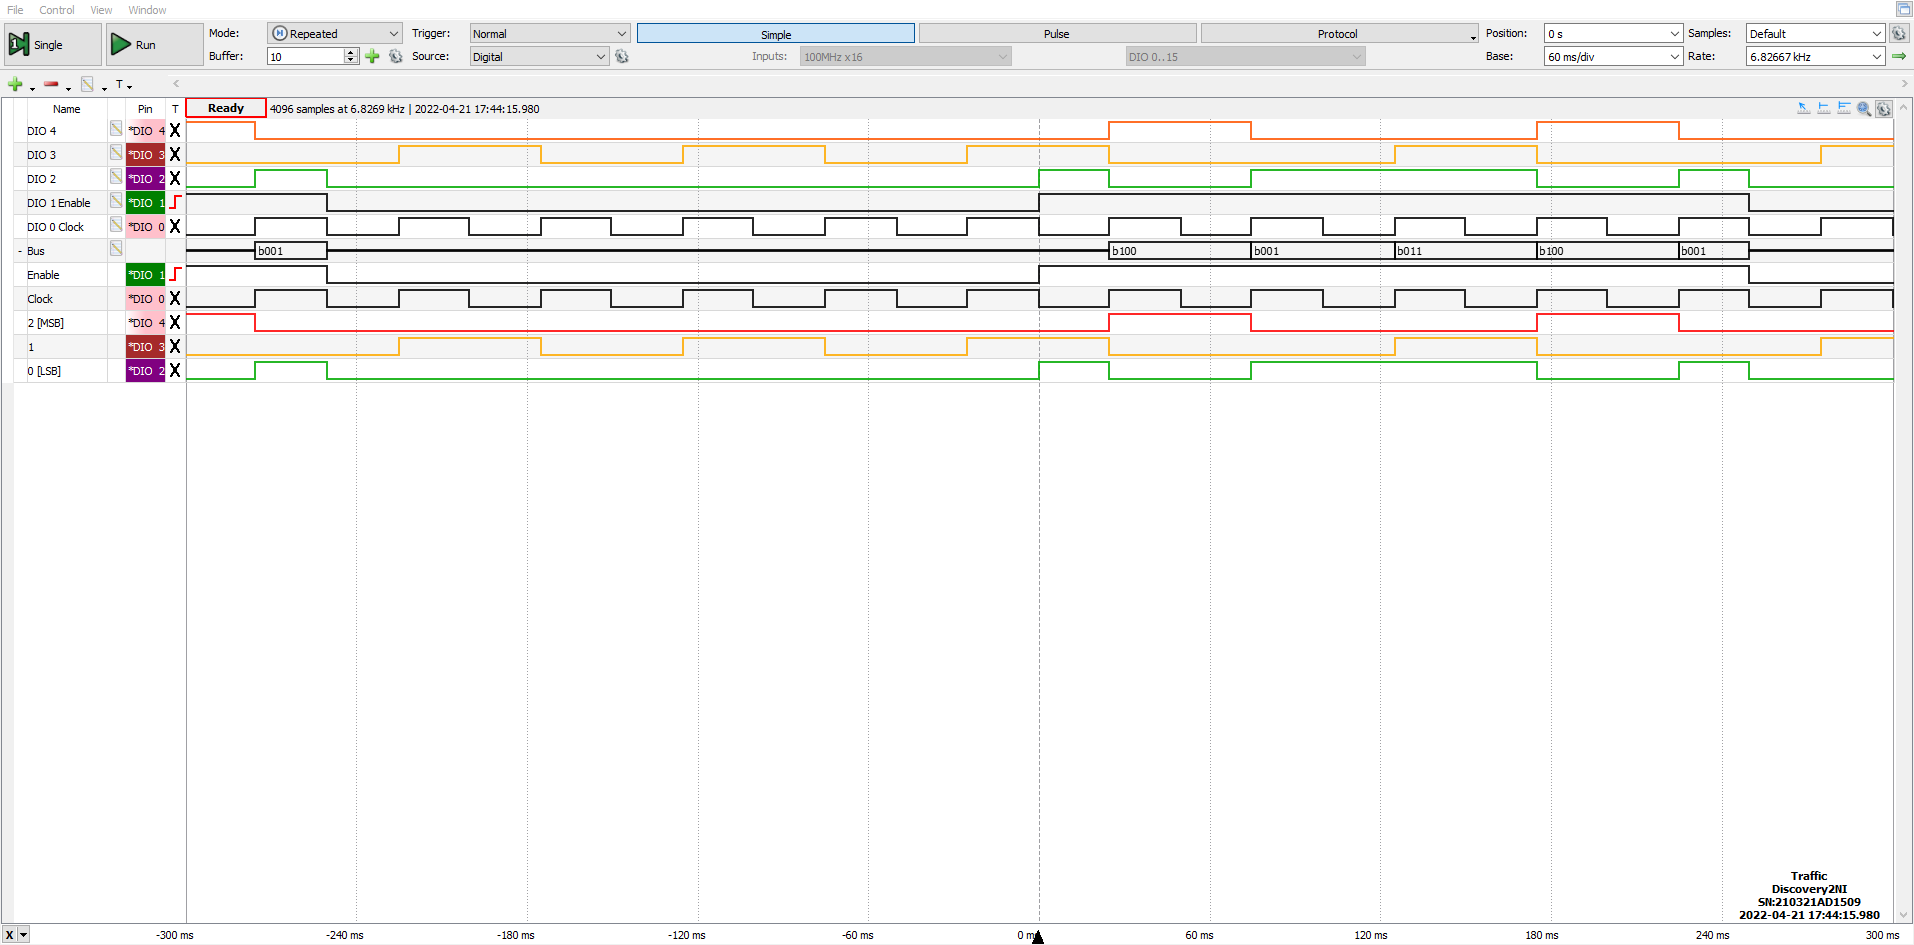
\includegraphics[width=\textwidth]{traffic}
    \caption{Acquisizione di un ciclo completo (frequenza 1 Hz) con Logic
    Analyzer dei segnali in ingresso e in uscita dal semaforo.
    \label{fig: traffic}}
\end{figure}

Osserviamo che, come atteso nel caso $E = 0$, $Q_0 = 1$ e $Q_1 = 0$ il
semaforo rimane rosso fino al fronte di salita successivo del clock prima
di spegnersi come previsto dalla modalità disabilitato.

%=======================
\section{Implementazione software della logica combinatoria con AD2/ROM}
\subsection{Costruzione del circuito}
Si vuole ricostruire il semaforo utilizzando la funzione ROM.
Come prima, andremo ad utilizzare 2 Flip-Flop per gestire i 3 stati del semaforo.
Dopo aver costruito il circuito in \cref{schem: rom} si va a programmare la ROM: innanzitutto si sono scelti ENABLE, Q0 e Q1 come input, per controllare lo stato corrente e se il semaforo risulta essere abilitato, e D0, D1 e gli ingressi ai LED come Output, in modo da sovrascrivere lo stato corrente e per accendere o spengere i led.
\begin{figure}[htbp]
    \centering
    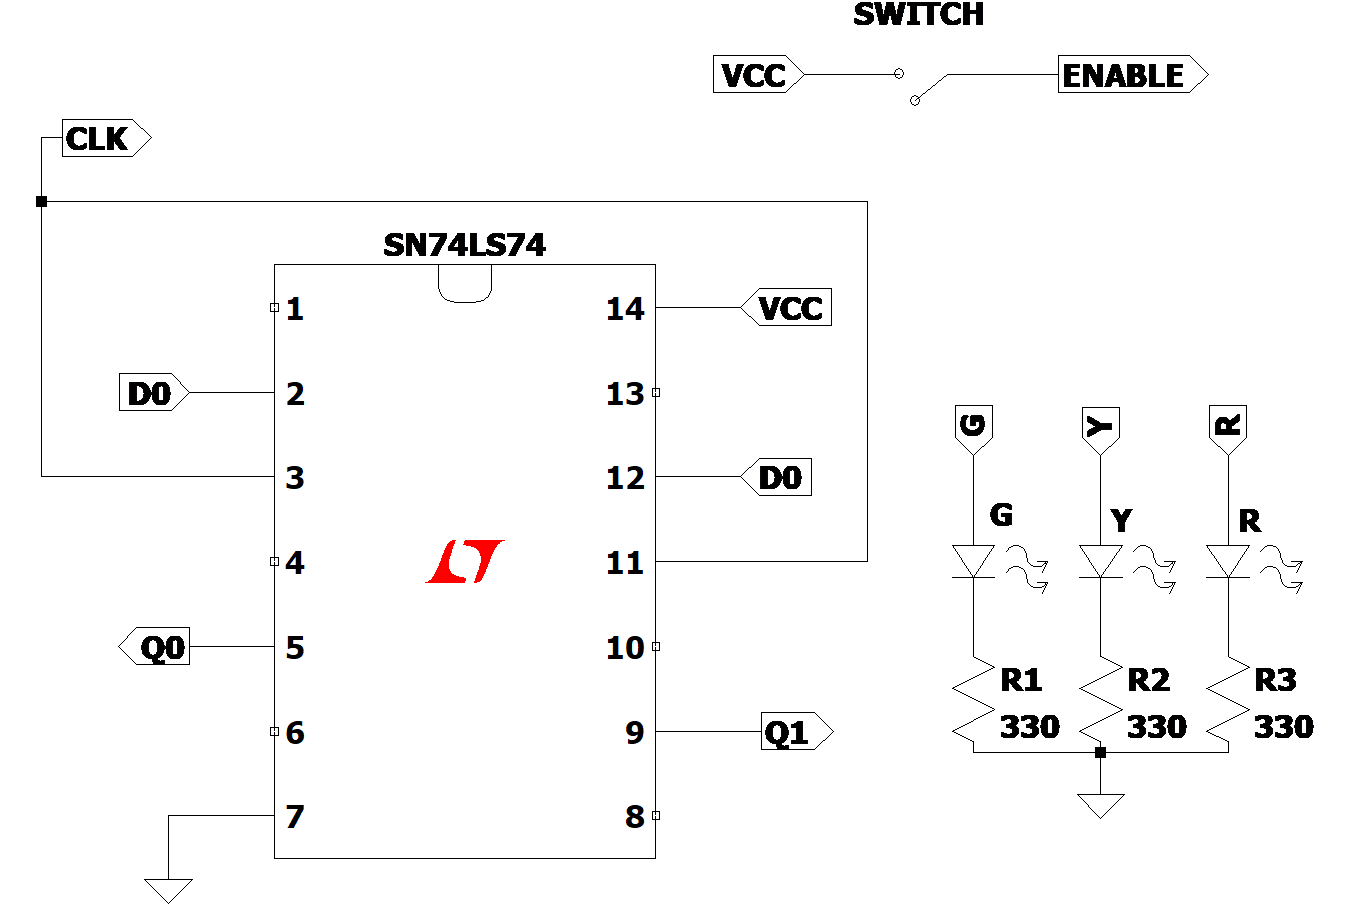
\includegraphics[width=\textwidth]{schem_rom}
    \caption{Schematica del circuito utilizzato per il semaforo gestito da ROM
    \label{schem: rom}}
\end{figure}

\subsection{Implementazione delle tabelle di verità in ROM}
Utilizzando la tabella di verità presente in \cref{tab: semftruth} abbiamo programmato la seguente ROM in cui è presente un unico stato illegale per entrami i funzionamenti (abilitato e disabilitato):
\begin{figure}[htbp]
    \centering
    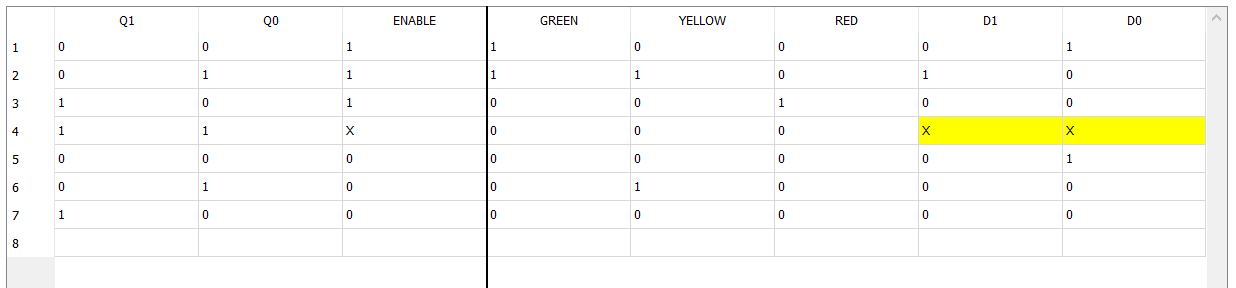
\includegraphics[width=\textwidth]{ROM.1}
    \caption{Tabella di verità programmata all'interno della ROM per il controllo del semaforo
    \label{fig: rom}}
\end{figure}

\subsection{Verifica del funzionamento del circuito}
Si procede quindi con la verifica del funzionamento del circuito.
Si invia al pin CLK un segnale di clock con frequenza pari ad 1 Hz, mantenendo collegati CLEAR e PRESET a Vcc come prima, e impostando la frequenza della ROM a 1 Mhz.
\begin{figure}[htbp]
    \centering
    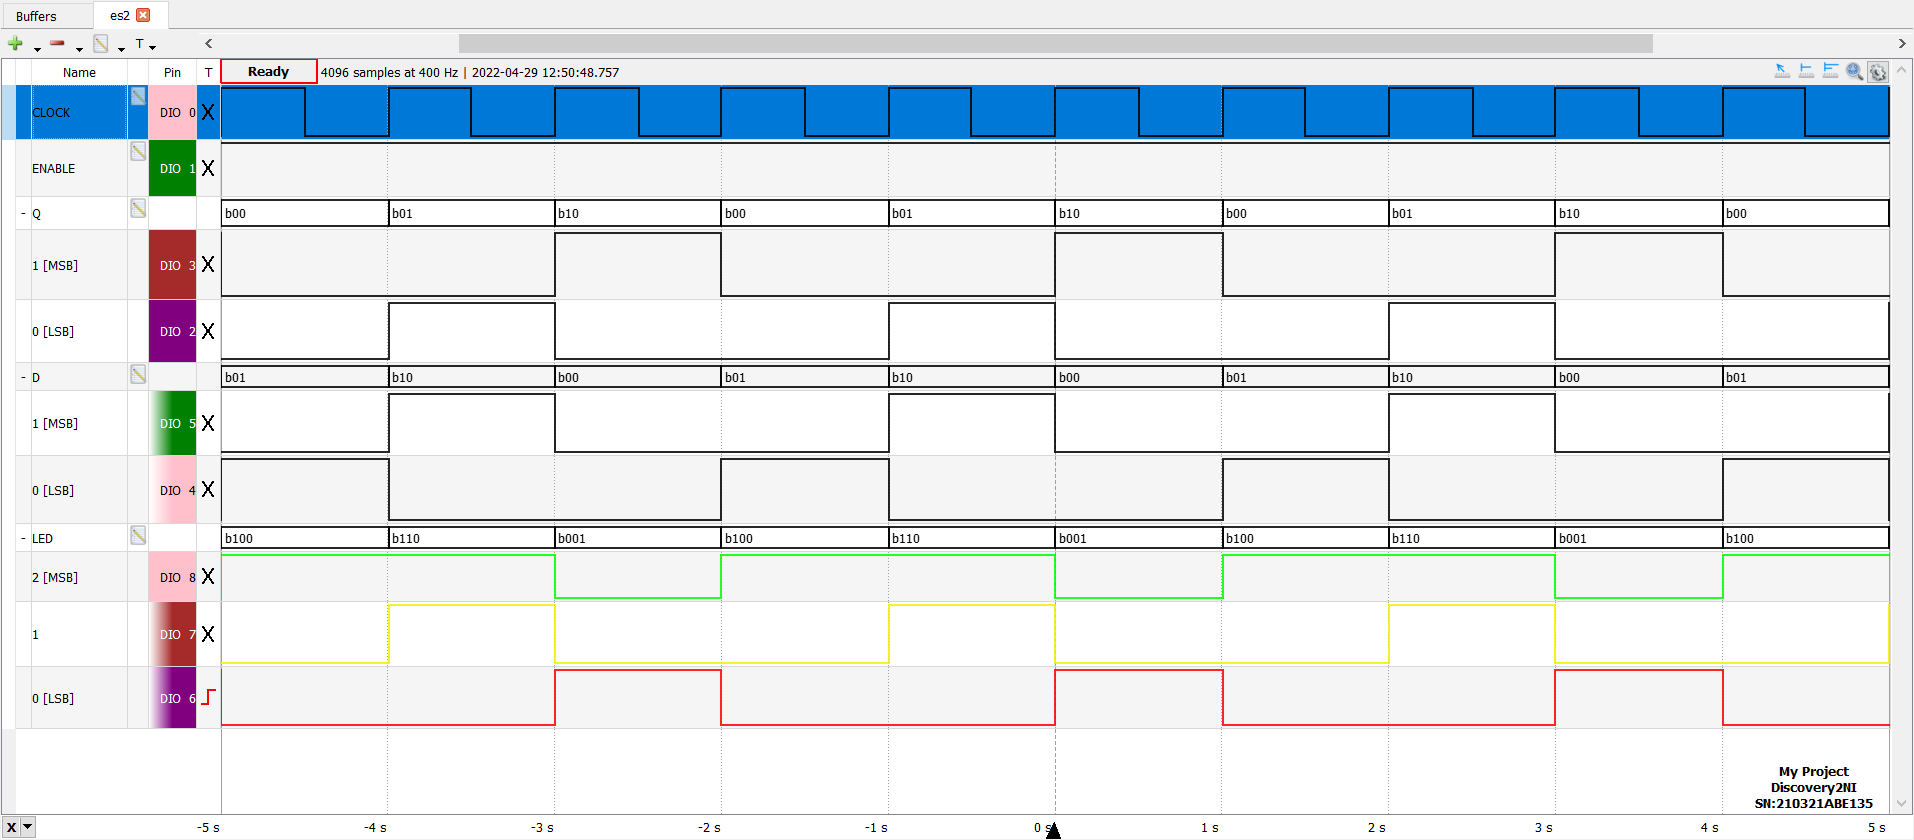
\includegraphics[width=\textwidth]{es2.enable}
    \caption{Acquisizione Logic del semaforo gestito da ROM, Abilitato
    \label{fig: es.2_enable}}
\end{figure}
\begin{figure}[htbp]
    \centering
    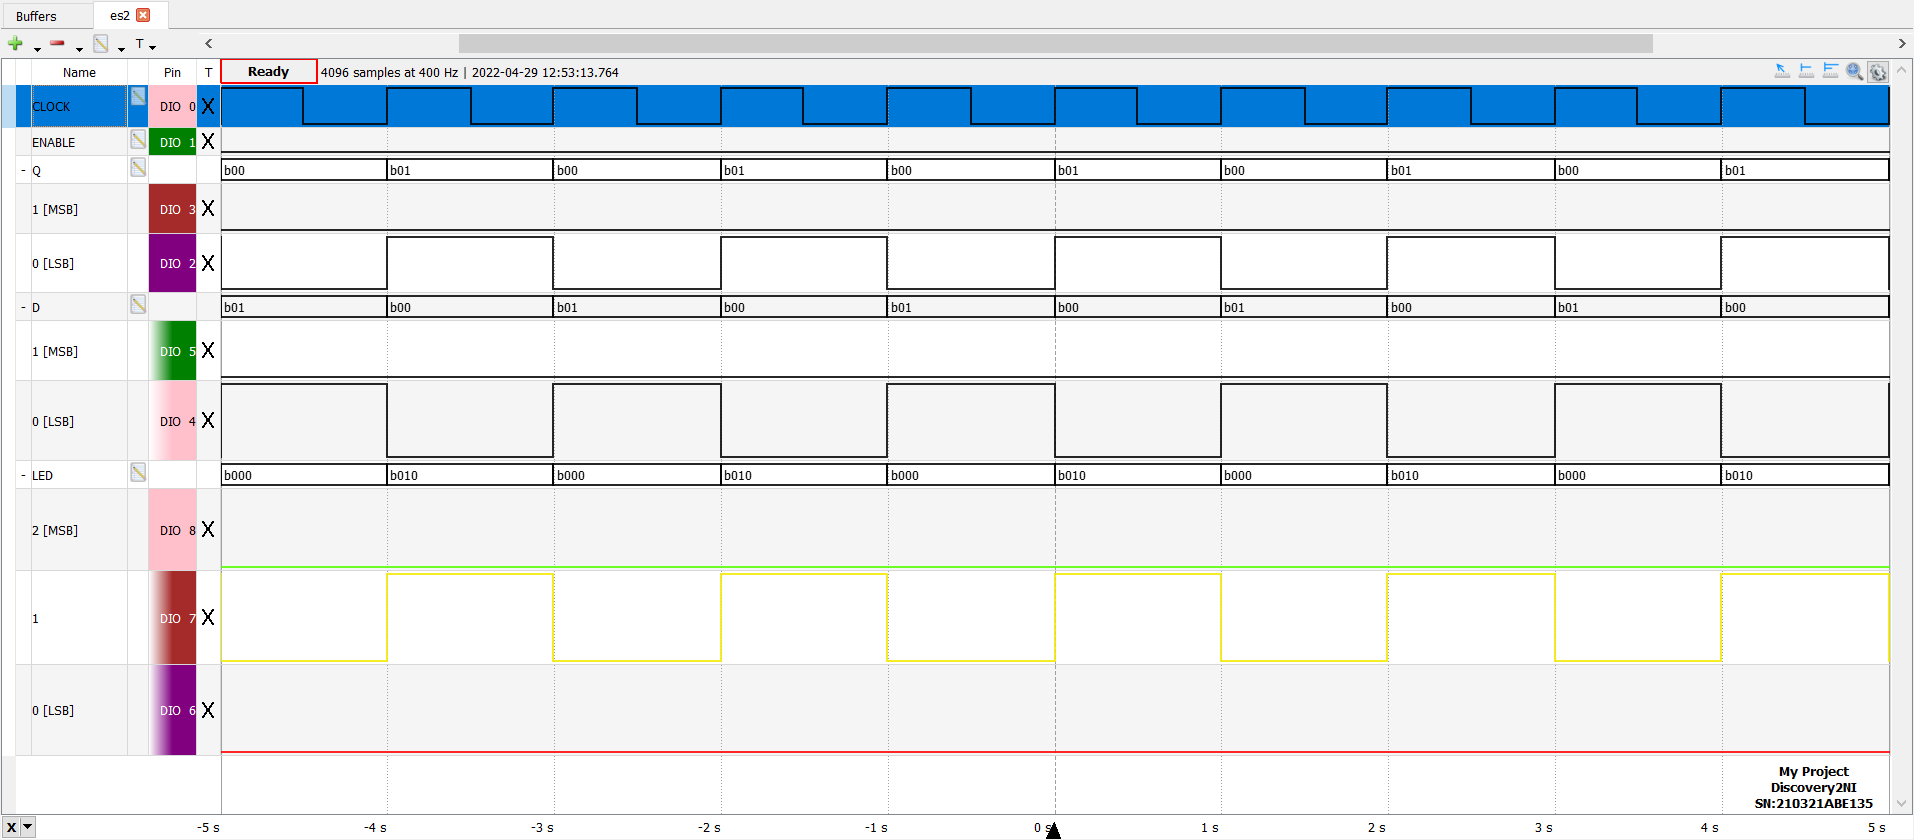
\includegraphics[width=\textwidth]{es2.disable}
    \caption{Acquisizione Logic del semaforo gestito da ROM, Disabilitato
    \label{fig: es.2_disable}}
\end{figure}
Dalle immagini \ref{fig: es.2_enable} e \ref{fig: es.2_disable} possiamo concludere che il circuito funzioni come da aspettativa.
\subsection{Variante svizzera del semaforo ROM}
Si va quindi a modificare la \cref{fig: rom} in modo da utilizzare anche lo stato $1\;1$ (successivo al rosso) per visualizzare lo stato rosso e giallo.
\begin{figure}[htbp]
    \centering
    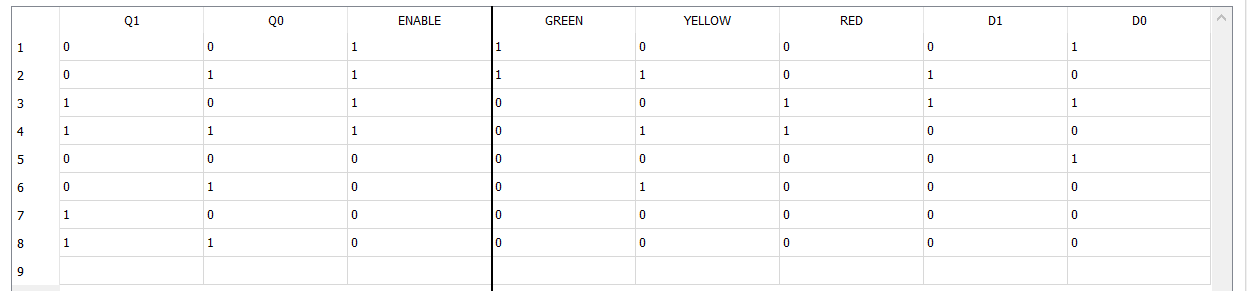
\includegraphics[width=\textwidth]{ROM.svizzero}
    \caption{Tabella di verità programmata all'interno della ROM per il controllo del semaforo svizzero
    \label{fig: rom.svizzero}}
\end{figure}
Si procede quindi a verificare il funzionamento del semaforo svizzero. Come prima inviamo un segnale di clock a 1 Hz e lasciamo la frequenza della ROM a 1 MHz.
\begin{figure}[htbp]
    \centering
    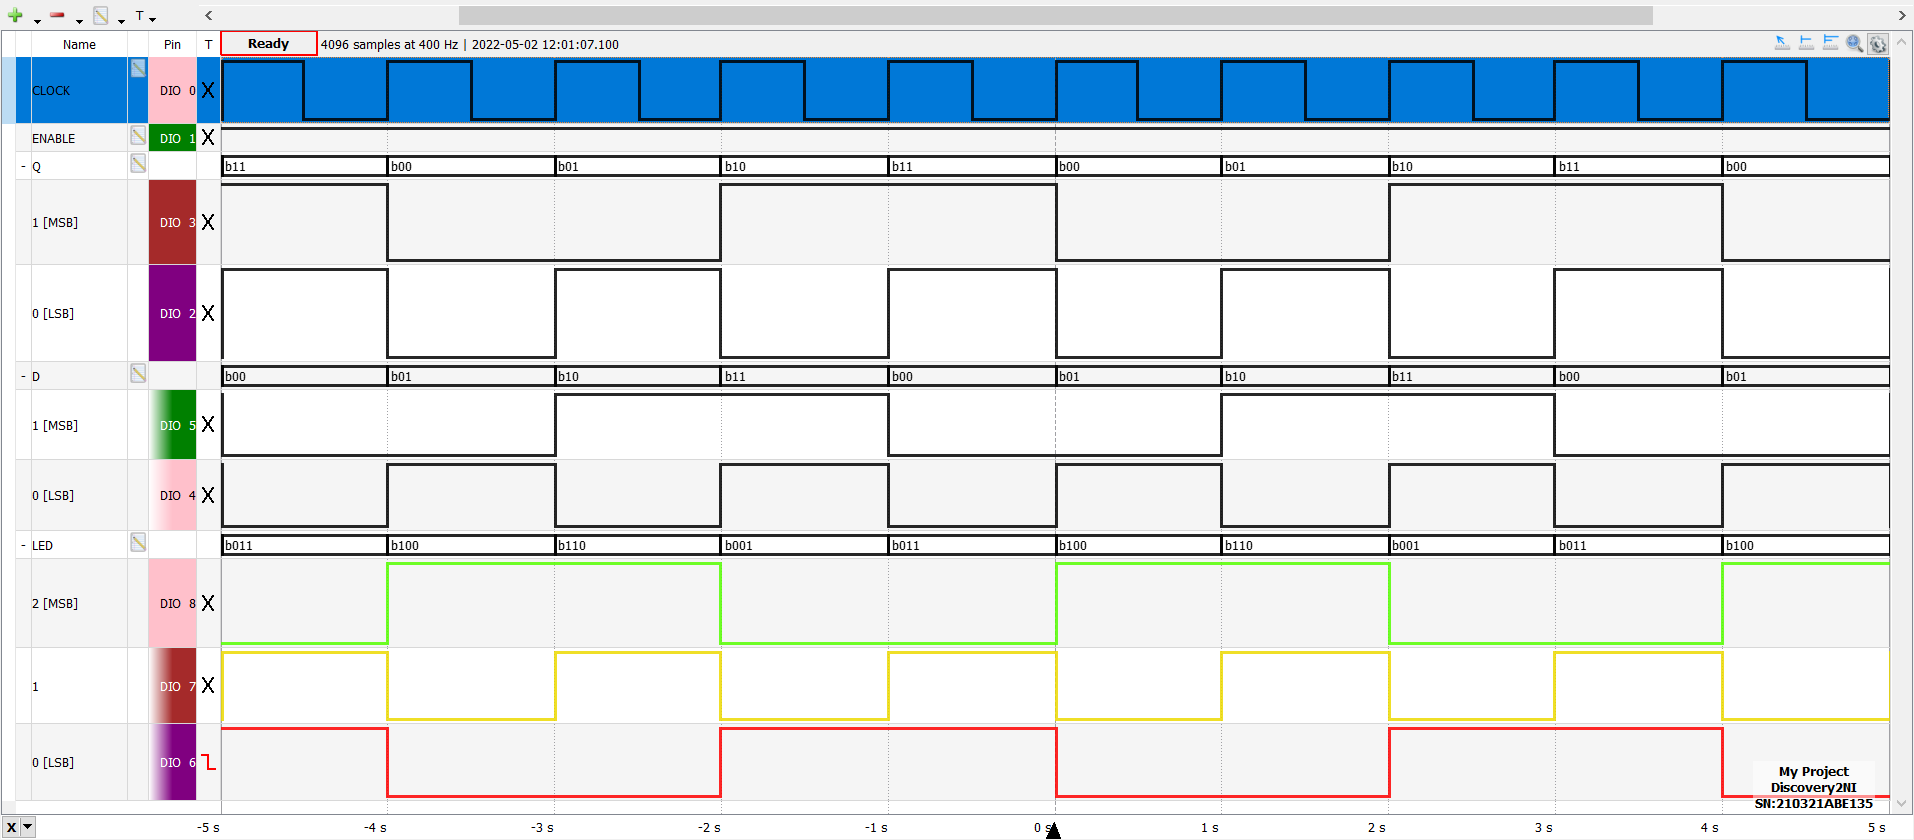
\includegraphics[width=\textwidth]{es2.svizzero}
    \caption{Acquisizione Logic del semaforo svizzero gestito da ROM, Abilitato
    \label{fig: es.2_svizzero}}
\end{figure}
Osservando la \cref{fig: es.2_svizzero} possiamo concludere che il circuito funziona come da aspettativa
%=======================
\section{Implementazione in software dei semafori con MCU (Arduino)}
Si vuole ricostruire il circuito precedente per il controllo di un semaforo tramite un microcontrollore (nel nostro caso utilizzeremo Arduino UNO).
\begin{figure}[htbp]
    \centering
    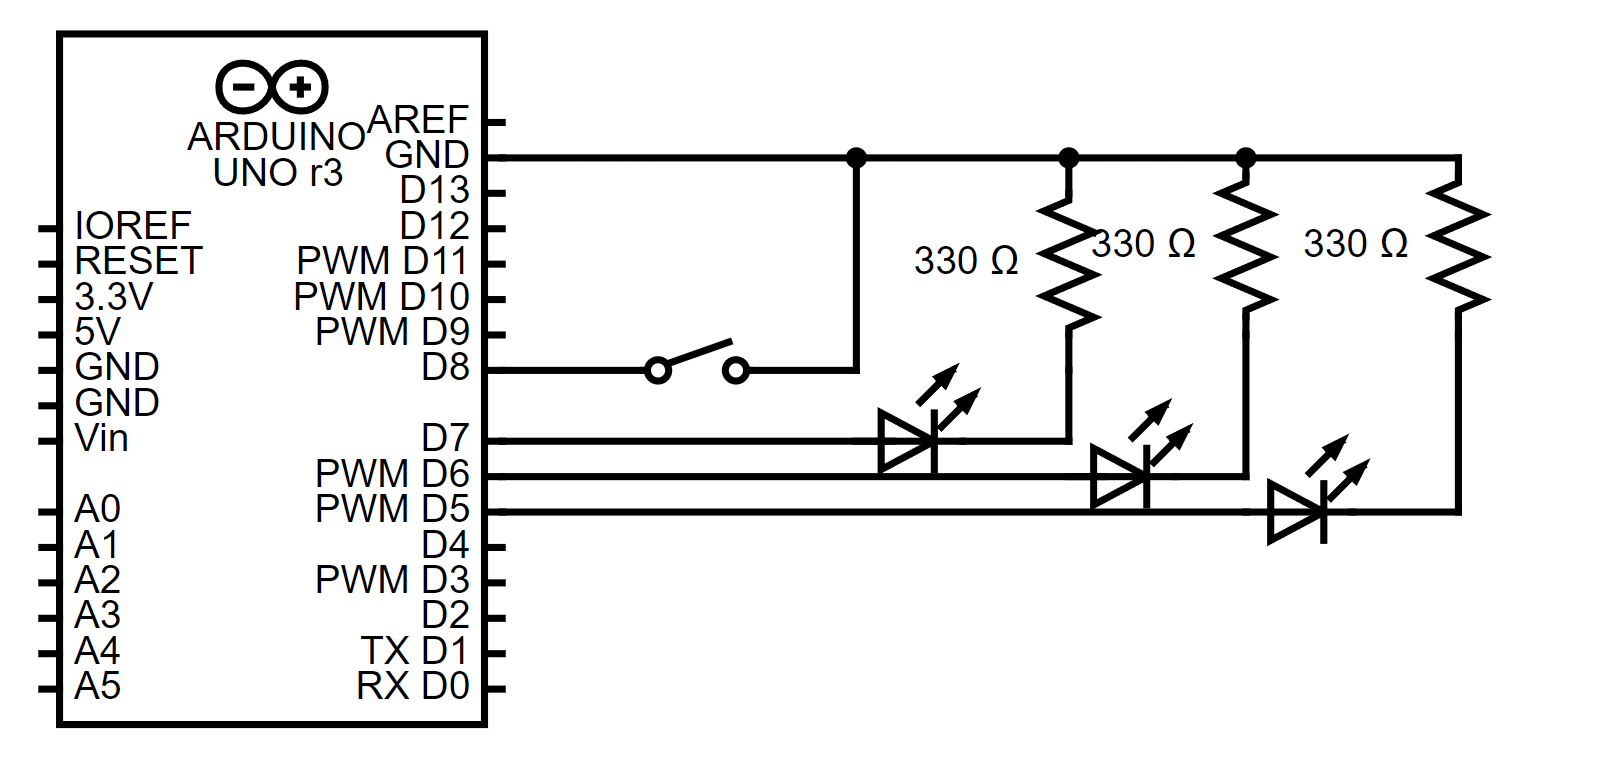
\includegraphics[width=\textwidth]{schem_ard}
    \caption{Schematica utilizzata nella gestione del semaforo con software tramite arduino.
    \label{schem: arduino}}
\end{figure}
Dopo aver montato il circuito descritto in \cref{schem: arduino}, si procede con l'implementazione software del semaforo.

\subsection{Implementazione del codice per la FSM}
Ci basiamo sullo schema per il semaforo FSM di Mealy presente in \cref{diag: semf} per controllare il funzionamento di un semaforo tramite enable.
\begin{lstlisting}[label={list:first}, style=Arduino, caption=Blink.ino]
/*state
 * 0= ALL OFF
 * 1= RED ON
 * 2= RED YELLOW ON
 * 3= GREEN ON
 * 4= GREEN YELLOW ON
 * 5= YELLOW ON
 * 
 */
void setup() {
  pinMode(5, OUTPUT); //Led Rosso
  pinMode(6, OUTPUT); //Led Giallo
  pinMode(7, OUTPUT); //Led Verde
  pinMode(8, INPUT_PULLUP); //Pin di Enable
}
int tickGREEN=1000; //Durata dello stato VERDE
int tickRED=1000; //Durata dello stato ROSSO
int tickYELLOW=1000; //Durata dello stato GIALLO
int tickREDYELLOW=1000; //Durata dello stato ROSSOGIALLO
int tickGREENYELLOW=1000; //Durata dello stato VERDEGIALLO
int tickOFF=1000; //Durata dello stato spento
int CurrentState=0; //stato iniziale impostato sul tutto spento

void loop() {
  //viene controllato se il semaforo \'e abilitato
  if(CheckEnable()){ 
    
    // nel caso in cui il semaforo sia abilitato
    switch(CurrentState){  

    case 1: //se lo stato precedente risulta essere rosso
      CurrentState=3; //lo stato corrente viene spostato a verde
      digitalWrite(5,LOW);
      digitalWrite(6,LOW);
      digitalWrite(7,HIGH);  
      delay(tickGREEN); //viene fatto trascorrere il tempo specificato all'inizio del file
      break; 
    case 3: //se lo stato precedente risulta essere solo verde
      CurrentState=4; //lo stato corrente viene portato a giallo e verde
      digitalWrite(6,HIGH);
      delay(tickGREENYELLOW);
      break;
      
    default: // in qualunque altro caso di stato precedente, se il semaforo \'e abilitato, lo stato inizializzato \'e quello rosso
      CurrentState=1;
      digitalWrite(5,HIGH);
      digitalWrite(6,LOW);
      digitalWrite(7,LOW);
      delay(tickRED); 
    }
    
  }else { 
    //nel caso in cui il semaforo sia disabilitato
    switch(CurrentState){
      case 5: // se lo stato precedente risulta essere giallo 
        CurrentState=0; //imposta lo stato corrente a tutto spento
        digitalWrite(6,LOW);
        delay(tickOFF); 
        break;     
      default: // in qualunque altro caso di stato precedente, lo stato inizializzato \'e quello giallo
        CurrentState=5;
        digitalWrite(6,HIGH);
        digitalWrite(5,LOW);
        digitalWrite(7,LOW);
        delay(tickYELLOW);
      }
  }
}

bool CheckEnable(){ 
  //Algoritmo di controllo per Enable
  
  int check =digitalRead(8);
  return (check== HIGH);
}
\end{lstlisting}
\subsection{Versione svizzera del semaforo con Enable via Arduino}
Si introduce un quarto stato nel caso in cui il semaforo sia abilitato, successivo al rosso; per fare ciò è necessaria una semplice modifica all'interno dello switch nel caso in cui il semaforo risulti abilitato
\begin{lstlisting}[label={list:first}, style=Arduino, caption=Blink.ino]
void loop() {
  //viene controllato se il semaforo \'e abilitato
  if(CheckEnable()){ 
    
    // nel caso in cui il semaforo sia abilitato
    switch(CurrentState){  
    case 1://se lo stato precedente risulta essere solo rosso
      CurrentState=2;
      digitalWrite(6,HIGH); //imposta lo stato corrente a rosso e giallo
      delay(tickREDYELLOW); //viene fatto passare il tempo specificato all'inizio del file
      break;
    case 2: //se lo stato precedente risulta essere rosso e giallo
      CurrentState=3; //lo stato corrente viene spostato a verde
      digitalWrite(5,LOW);
      digitalWrite(6,LOW);
      digitalWrite(7,HIGH);  
      delay(tickGREEN); 
      break; 
    .
    .
    .
\end{lstlisting}
%=======================
\section{Falling-edge detector}
Si vuole realizzare una FSM che riceve uno stream di bit su una linea di
ingresso e che accende un LED tutte le volte che su questo si presenta un
fronte di discesa secondo il modello di Moore e un'altra secondo quello di
Mealy.
\subsection{Progettazione FSM e costruzione dei circuiti}
Come nella \ref{sec: IC}
\begin{figure}[htbp]
\centering
\begin{FSM}
\tikzset{node distance = 4cm, on grid, auto
}
\node (H) [state with output] {HIGH \nodepart{lower} $01$};
\node (C) [state with output, right of = H] {EDGE \nodepart{lower} $10$};
\node (L) [state with output, right of = C] {LOW \nodepart{lower} $00$};
 
\path [-stealth, thick]
	(H) edge [loop left]  node {IN=1}()
    (H) edge [bend left] node[above] {IN=0} (C)
    (C) edge [bend left] node[above] {IN=1} (H)
    (C) edge [bend left] node[above] {IN=0} (L)
    (L) edge [bend left] node {IN=1} (H)
    (L) edge [loop right]  node {IN=0}();
\end{FSM}
\caption{Edge detector FSM di Moore
\label{diag: edgeMoore}}
\end{figure}

\begin{table}[htbp]
\centering
\begin{tabular}{c:c|cc||cc|c}
\toprule
State & IN & $Q_1$ & $Q_0$ & $D_1$ & $D_0$ & OUT \\
\midrule
\midrule
LOW   & 0  & 0  & 0  & 0  & 0  & 0   \\
      & 1  & 0  & 0  & 0  & 1  & 0   \\
\midrule
EDGE  & 0  & 1  & 0  & 0  & 0  & 1   \\
      & 1  & 1  & 0  & 0  & 1  & 1   \\
\midrule
HIGH  & 0  & 0  & 1  & 1  & 0  & 0   \\
      & 1  & 0  & 1  & 0  & 1  & 0   \\
\bottomrule
\end{tabular}
\caption{codifica binaria degli stati del detector di Moore.
\label{tab: bitMoore}}
\end{table}

\begin{table}[htbp]
\centering
	\begin{tabular}{c|c|c|c|c}
        \backslashbox{IN}{$Q_1 Q_0$} & 00 & 01 & 11 & 10\\
        \hline
        0 & 0 & 0 & X & 0 \\
        \hline
        1 & 1 & 1 & X & 1 \\
    \end{tabular}
	\caption{Tabella di Karnaugh per $D_0 = \text{IN}$
	 \label{tab: KarD0edge}}

\bigskip
	 
    \begin{tabular}{c|c|c|c|c}
        \backslashbox{IN}{$Q_1 Q_0$} & 00 & 01 & 11 & 10\\
        \hline
        0 & 0 & \cellcolor[HTML]{FF9999} 1 & \cellcolor[HTML]{FF9999} X & 0 \\
        \hline
        1 & 0 & 0 & X & 0 \\
    \end{tabular}
	\caption{Tabella di Karnaugh per $D_1 = \overline{\text{IN}} \cdot Q_0$
	 \label{tab: KarD1edge}}

\bigskip

    \begin{tabular}{c|c|c|c|c}
        \backslashbox{IN}{$Q_1 Q_0$} & 00 & 01 & 11 & 10\\
        \hline
        0 & 0 & 0 & \cellcolor[HTML]{FF9999} X & \cellcolor[HTML]{FF9999} 1 \\
        \hline
        1 & 0 & 0 & \cellcolor[HTML]{FF9999} X & \cellcolor[HTML]{FF9999} 1 \\
    \end{tabular}
    \caption{Tabella di Karnaugh per $\text{OUT} = Q_1$
    \label{tab: KarOUT}}
\end{table}

\begin{figure}[htbp]
    \centering
    \begin{circuitikz}
    \tikzset{flipflop D/.style={flipflop,
    flipflop def={t1=$D_0$, t6=$Q_0$, c3=1, t4=\ctikztextnot{$Q_0$}}},
	}
        \def\andScale{0.7};

        % componenti
        %% flip flop
        \draw (0,0) node[flipflop D] (ffSinistra) {};
		\tikzset{flipflop D/.style={flipflop,
		flipflop def={t1=$D_1$, t6=$Q_1$, c3=1, t4=\ctikztextnot{$Q_1$}}},
		}
        \draw (5,0) node[flipflop D] (ffDestra) {};
        
        %% and gate
        \node (andDestra) at (3, |- ffDestra.pin 1) [and port, scale=\andScale] {};
        \node at (andDestra.bin 1) [ocirc, left] {};
        
        % input
        \node (IN) at ($ (ffSinistra.pin 1) + (-2,1) $) {IN};
        \node (CLK) at ($ (IN) + (0,-4) $) {CLK};
        \draw (9.5,-1.5) node[eground] (gnd){};

        % fili
        %% clock e in
        \draw (CLK) -| (ffDestra.pin 3);
        \draw (ffSinistra.pin 3) -- (ffSinistra.pin 3 |-, |- CLK);
        \draw (IN) -| (andDestra.in 1);
        \draw (ffSinistra.pin 1) -- (ffSinistra.pin 1 |-, |- IN);
        \draw (ffSinistra.pin 6) |- (andDestra.in 2);
        
        \draw (andDestra.out) -- (ffDestra.pin 1);
        \draw (ffDestra.pin 6) to
        [/tikz/circuitikz/bipoles/length=1cm,empty led, l=OUT]
        ++ (1.5,0) to[/tikz/circuitikz/bipoles/length=1cm, R,l=\SI{1}{\kilo\ohm}]
        ++ (1.5,0) -| (gnd);
    \end{circuitikz}
    \caption{schema del detector Moore.
    \label{schm: edgeMoore}}
\end{figure}

\begin{figure}[htbp]
\centering
\begin{FSM}
\tikzset{node distance = 4cm, on grid, auto
}
\node (H) [state] {HIGH};
\node (L) [state, right of = H] {LOW};
 
\path [-stealth, thick]
	(H) edge [loop left]  node {IN$=1$ (OUT$=0$)}()
    (H) edge [bend left] node[above] {IN$=0$ (OUT$=1$)} (L)
    (L) edge [bend left] node {IN$=1$ (OUT$=0$)} (H)
    (L) edge [loop right]  node {IN$=0$ (OUT$=0$)}();
\end{FSM}
\caption{Edge detector FSM di Mealy
\label{diag: edgeMealy}}
\end{figure}

\begin{table}[htbp]
	\centering
	\begin{tabular}{cc|c}
	\toprule
	$D$ = IN & $Q$ & OUT \\
	\midrule
	\midrule
	$0$  & $0$	& $0$ \\
	$0$  & $1$	& $1$ \\
	$1$  & $0$	& $0$ \\
	$1$  & $1$  & $0$ \\
	\bottomrule
	\end{tabular}
	\caption{codifica binaria degli stati del detector di Mealy.
	$D$ = IN; OUT = $\overline{\text{IN}} \cdot Q$
	\label{tab: bitMealy}}
\end{table}

\begin{figure}[htbp]
    \centering
    \begin{circuitikz}
	\def\andScale{0.7};
        % componenti
        %% flip flop
        \draw (0,0) node[flipflop D] (ffSinistra) {};
        
        %% and gate
        \node (andDestra) at ($ (ffSinistra.pin 6) + (1.5,0.2) $) [and port, scale=\andScale] {};
        \node at (andDestra.bin 1) [ocirc, left] {};
        
        % input
        \node (IN) at ($ (ffSinistra.pin 1) + (-2,1) $) {IN};
        \node (CLK) at ($ (ffSinistra.pin 3) + (-2,0) $) {CLK};
        \draw (6.5,-1) node[eground] (gnd){};

        % fili
        %% clock e in
        \draw (CLK) -| (ffSinistra.pin 3);
        \draw (IN) -| (andDestra.in 1);
        \draw (ffSinistra.pin 1) -- (ffSinistra.pin 1 |-, |- IN);
        \draw (ffSinistra.pin 6) |- (andDestra.in 2);
        
        \draw (andDestra.out) to
        [/tikz/circuitikz/bipoles/length=1cm,empty led, l=OUT]
        ++ (1.5,0) to[/tikz/circuitikz/bipoles/length=1cm, R,l=\SI{1}{\kilo\ohm}]
        ++ (1.5,0) -| (gnd);
    \end{circuitikz}
    \caption{schema del detector Mealy.
    \label{schm: edgeMealy}}
\end{figure}

\subsection{Definizione dello stream di bit casuali in ingresso}
Con la funzione Patterns di Waveform si invia un segnale (in DIO 5) di clock
di frequenza $f\ped{clk} = \SI{1}{k\Hz}$ al pin (CLK) dei Flip-Flop e si
genera con il canale DIO 6 uno stream di dati random alla stessa frequenza
$f = f\ped{clk}$, già dalla schermata di Patterns è possibile notare come
le commutazioni di stato del segnale pseudocasuale avvengano in corrispondenza
dei fronti di discesa del segnale di clock.

Come prima si sono mantenuti i pin PRESET e CLEAR dei D-FF collegati a
$V_{CC}$ per evitare reset o clear spuri.

\subsection{Verifica del funzionamento e analisi della temporizzazione}
Si sono acquisiti i segnali in ingresso (CLK = DIO 5, IN = DIO 6) e in uscita
(OUT = DIO 7) dai circuiti edge-detector con la funzione Logic Analyzer
dell'AD2, di cui riportiamo i risultati per il circuito di Moore in
\cref{fig: edgeMoore} e per la FSM di Mealy in \cref{fig: edgeMealy}.
\begin{figure}[htbp]
    \centering
    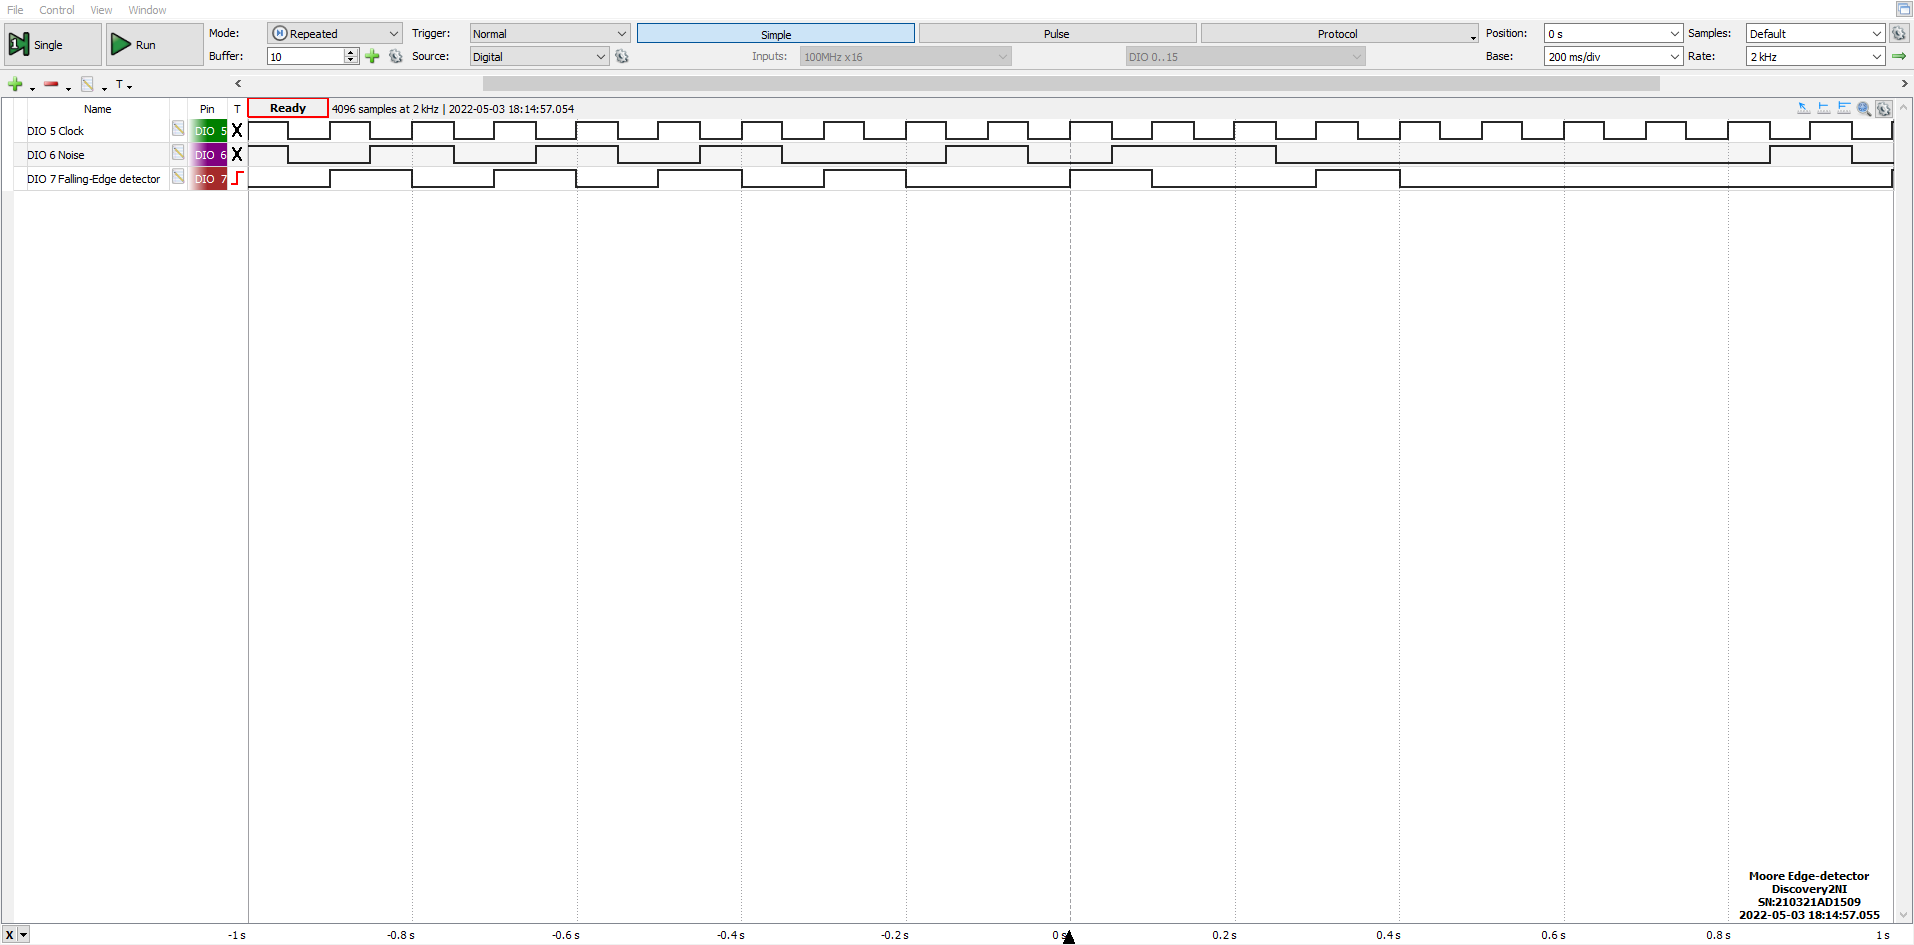
\includegraphics[width=\textwidth]{Moore_edge_detector}
    \caption{Acquisizione di un ciclo completo (frequenza 1 kHz) con Logic
    Analyzer dei segnali in ingresso e in uscita dall'edge detector di Moore.
    \label{fig: edgeMoore}}
\end{figure}
Notiamo nel primo caso come l'uscita assume valore alto in maniera sincrona
rispetto al segnale di clock, mentre nell'implementazione di Mealy l'uscita
non aspetta il successivo fronte d'onda del clock per salire al livello logico
alto e accendere il LED.
\begin{figure}[htbp]
    \centering
    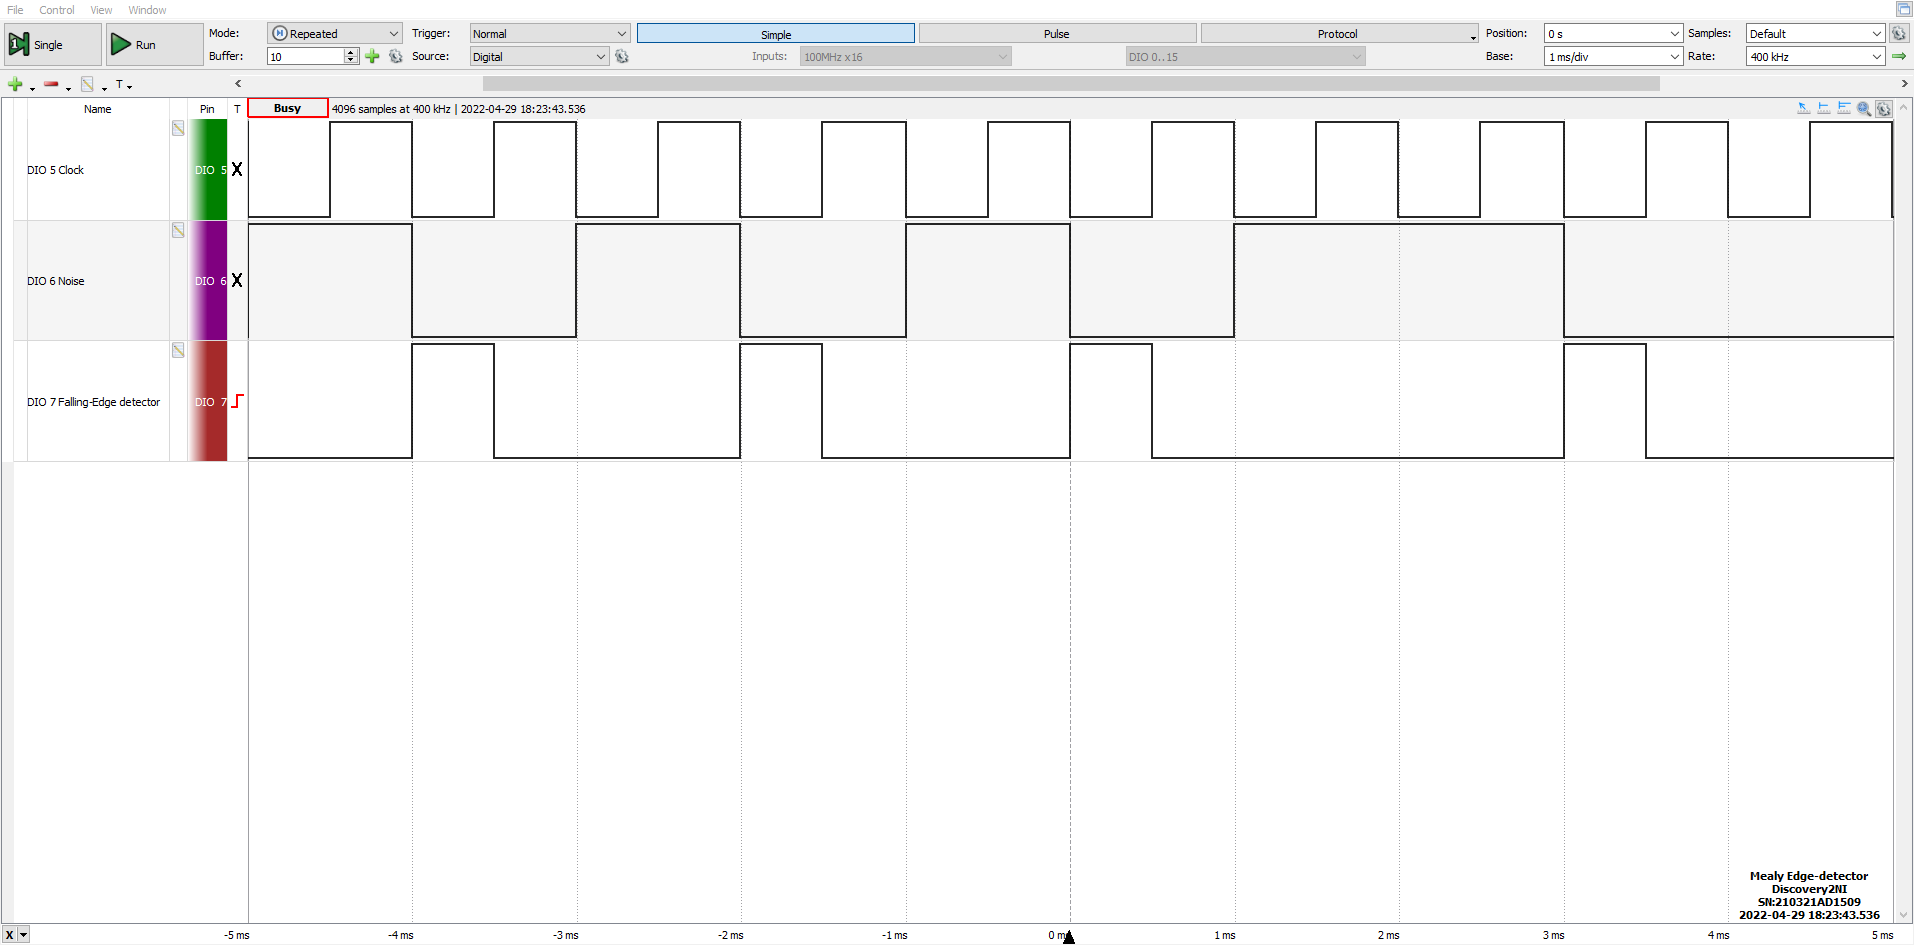
\includegraphics[width=\textwidth]{Mealy_edge_detector}
    \caption{Acquisizione di un ciclo completo (frequenza 1 kHz) con Logic
    Analyzer dei segnali in ingresso e in uscita dal detector di Mealy.
    \label{fig: edgeMealy}}
\end{figure}

%=======================
\section*{Conclusioni e commenti finali}
Si è riusciti a progettare, costruire e verificare il corretto funzionamento
di circuiti logici combinatori di diversa complessità e svariate applicazioni
(e.g., sistemi di controllo e misura) costruiti con porte NOT, NAND, OR e D-FF.
Inoltre si è riusciti ad apprezzare le diverse modalità di funzionamento delle
macchine a stati finiti implementate secondo i modelli Moore e Mealy, ponendo
particolare attenzione alle loro diverse temporizzazioni nei cambiamenti di
stato, nonostante la bassa risoluzione temporale dell'AD2.

%=======================
\section*{Dichiarazione}
I firmatari di questa relazione dichiarano che il contenuto della relazione \`e
originale, con misure effettuate dai membri del gruppo, e che tutti i firmatari
hanno contribuito alla elaborazione della relazione stessa.

\end{document}
